\documentclass[tikz,border=10pt]{standalone}
\usepackage{amsmath}

\begin{document}

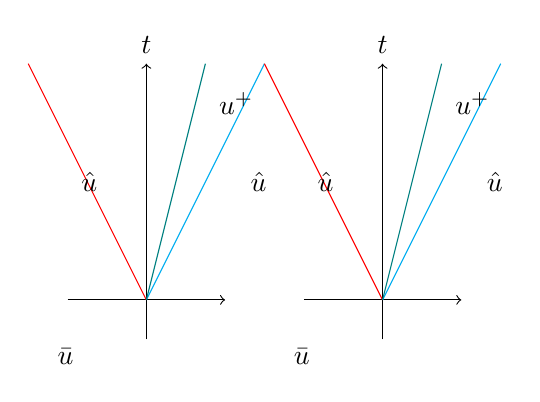
\begin{tikzpicture}
    % Left Diagram
    \begin{scope}
        % Axes
        \draw[->] (0,-0.5) -- (0,3) node[above] {$t$};
        \draw[->] (-1,0) -- (1,0);
        
        % Wave fronts
        \draw[red] (0,0) -- (-1.5,3);
        \draw[cyan] (0,0) -- (1.5,3);
        \draw[teal] (0,0) -- (0.75,3);

        % Labels
        \node at (-0.5,1.5) [anchor=east] {$\hat{u}$};
        \node at (1.2,1.5) [anchor=west] {$\hat{u}$};
        \node at (0.8,2.5) [anchor=west] {$u^+$};
        \node at (-0.8,-0.5) [anchor=north east] {$\bar{u}$};
    \end{scope}
    
    % Right Diagram
    \begin{scope}[xshift=3cm]
        % Axes
        \draw[->] (0,-0.5) -- (0,3) node[above] {$t$};
        \draw[->] (-1,0) -- (1,0);
        
        % Wave fronts
        \draw[red] (0,0) -- (-1.5,3);
        \draw[cyan] (0,0) -- (1.5,3);
        \draw[teal] (0,0) -- (0.75,3);

        % Labels
        \node at (-0.5,1.5) [anchor=east] {$\hat{u}$};
        \node at (1.2,1.5) [anchor=west] {$\hat{u}$};
        \node at (0.8,2.5) [anchor=west] {$u^+$};
        \node at (-0.8,-0.5) [anchor=north east] {$\bar{u}$};
    \end{scope}
\end{tikzpicture}

\end{document}